%%%%% VisIt
%\section{VisIt}
\subsection{Generalities}
\begin{frame}
\frametitle{\href{https://wci.llnl.gov/simulation/computer-codes/visit/}{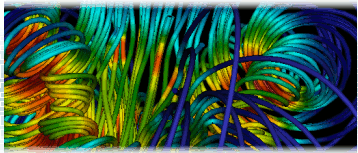
\includegraphics[height=.85cm]{figs/visit-logos/VisIt-01}} \href{https://wci.llnl.gov/simulation/computer-codes/visit/}{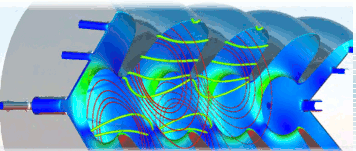
\includegraphics[height=.875cm]{figs/visit-logos/VisIt-02}} \href{https://wci.llnl.gov/simulation/computer-codes/visit/}{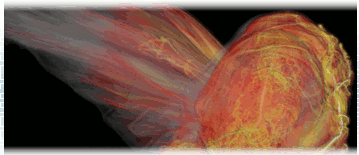
\includegraphics[height=.875cm]{figs/visit-logos/VisIt-03}} \href{https://wci.llnl.gov/simulation/computer-codes/visit/}{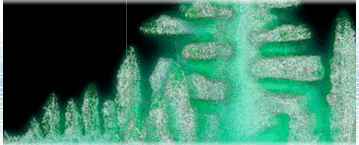
\includegraphics[height=.875cm]{figs/visit-logos/VisIt-04}} \hspace{-8.5cm}{\bf \textcolor{white}{VisIt}}}

%\vspace{-5mm}
%\hspace{-2.5mm}
%\href{https://wci.llnl.gov/simulation/computer-codes/visit}{\textcolor{DarkBlue}{\small\tt https://wci.llnl.gov/simulation/computer-codes/visit}}
%
%\hspace{-2.5mm}
%\href{http://visit.llnl.gov/}{\textcolor{DarkBlue}{\tt http://visit.llnl.gov/}}

\vspace{-3.5mm}
\begin{columns}%[T]
\begin{column}{7.65cm}
\vspace{-2mm}
\href{https://wci.llnl.gov/simulation/computer-codes/visit}{\textcolor{DarkBlue}{\small\tt https://wci.llnl.gov/simulation/computer-codes/visit}}

\href{http://visit.llnl.gov/}{\textcolor{DarkBlue}{\tt http://visit.llnl.gov/}}

\begin{small}
\begin{itemize}
        \item Developed by the \textit{DOE Advanced Simulation and Computing Initiative}, %(ASCI)
 to visualize results of terascale simulations, first release fall of 2002 -- mantained by \textit{LLNL}
        \item \textcolor{DarkRed}{v2.10.2} \href{https://wci.llnl.gov/simulation/computer-codes/visit/downloads}{available as source and binary for \textcolor{DarkBlue}{Linux/Mac/Windows}}
        \item Over 80 visualization features (contour, mesh, slice, volume, molecule, ...)
        %\item Reads over 120 different file formats (\ding{223} \href{http://www.visitusers.org/index.php?title=Detailed_list_of_file_formats_VisIt_supports}{\small detailed list of file formats})
        \item Interfaces with C++, Python, and Java
        \item Uses MPI for \textcolor{DarkBlue}{distributed-memory parallelism} on HPC clusters
\end{itemize}
\end{small}
\end{column}
\begin{column}{5cm}
	\vspace{-2mm}

        \href{https://wci.llnl.gov/simulation/computer-codes/visit/gallery}{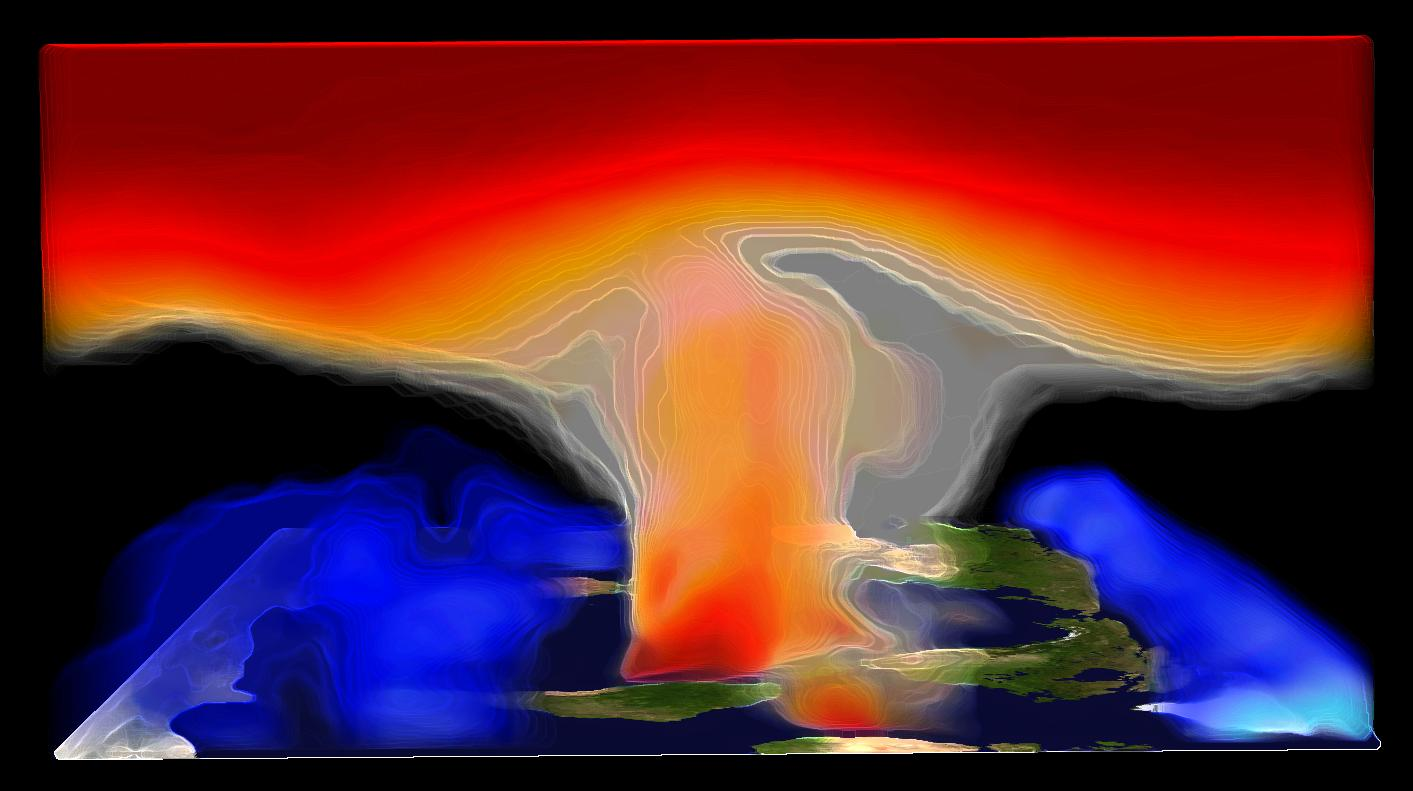
\includegraphics[width=.475\columnwidth]{figs/visit-exs/VisIt-gallery_33}}
        \href{https://wci.llnl.gov/simulation/computer-codes/visit/gallery}{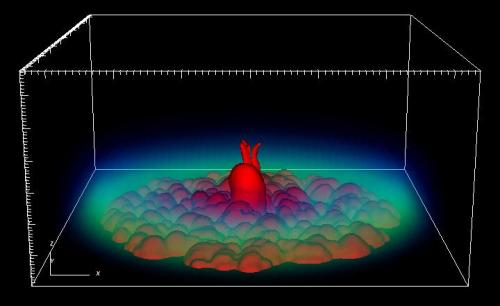
\includegraphics[width=.475\columnwidth]{figs/visit-exs/VisIt-gallery_10}}

        \href{https://wci.llnl.gov/simulation/computer-codes/visit/gallery}{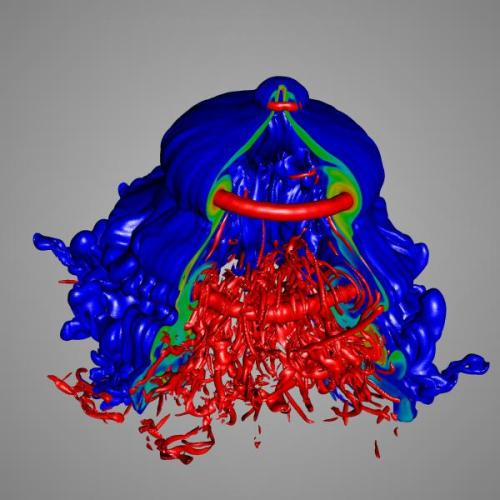
\includegraphics[width=.475\columnwidth]{figs/visit-exs/VisIt-gallery_00}}
        \href{https://wci.llnl.gov/simulation/computer-codes/visit/gallery}{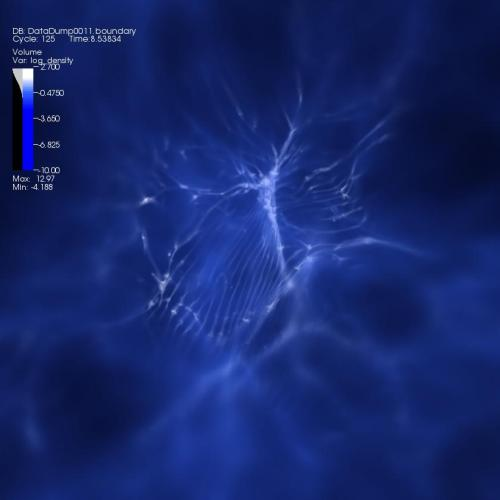
\includegraphics[width=.475\columnwidth]{figs/visit-exs/VisIt-gallery_05}}

        \href{https://wci.llnl.gov/simulation/computer-codes/visit/gallery}{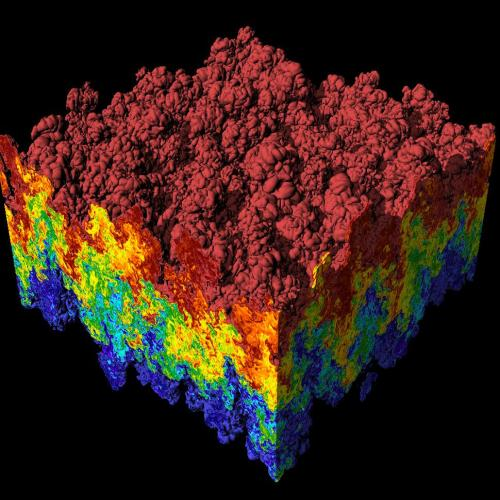
\includegraphics[width=.475\columnwidth]{figs/visit-exs/VisIt-gallery_02}}
        \href{https://wci.llnl.gov/simulation/computer-codes/visit/gallery}{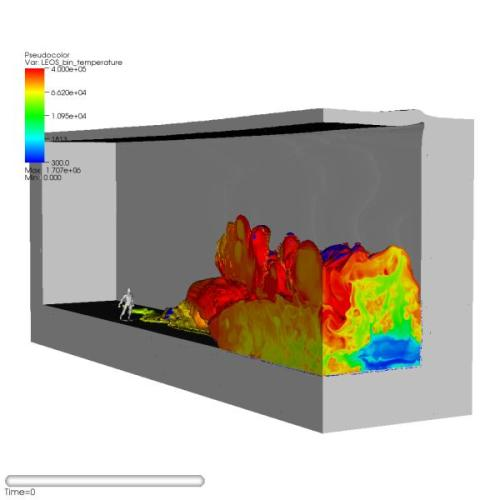
\includegraphics[width=.475\columnwidth]{figs/visit-exs/VisIt-gallery_01}}

        \href{https://wci.llnl.gov/simulation/computer-codes/visit/gallery}{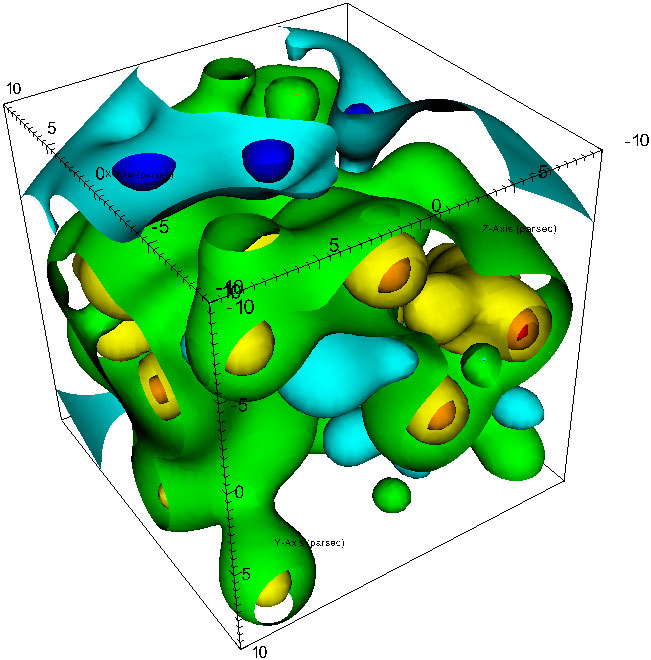
\includegraphics[width=.475\columnwidth]{figs/visit-exs/VisIt-contour1_S}}
        \href{https://wci.llnl.gov/simulation/computer-codes/visit/gallery}{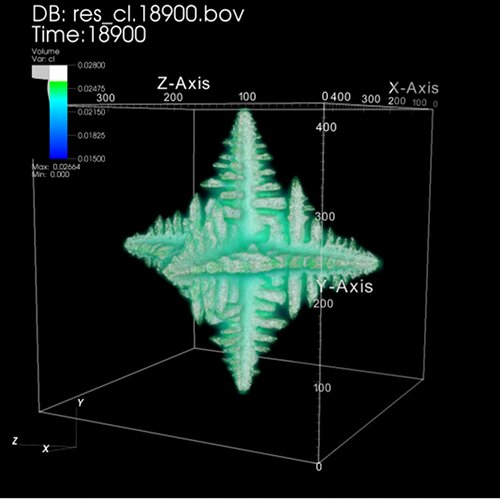
\includegraphics[width=.475\columnwidth]{figs/visit-exs/VisIt-gallery_39}}
\end{column}
\end{columns}
\end{frame}


\begin{frame}
\frametitle{\href{https://wci.llnl.gov/simulation/computer-codes/visit/}{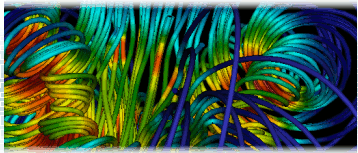
\includegraphics[height=.85cm]{figs/visit-logos/VisIt-01}} \href{https://wci.llnl.gov/simulation/computer-codes/visit/}{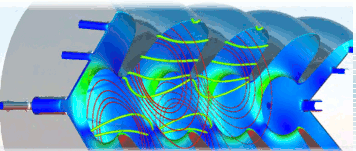
\includegraphics[height=.875cm]{figs/visit-logos/VisIt-02}} \href{https://wci.llnl.gov/simulation/computer-codes/visit/}{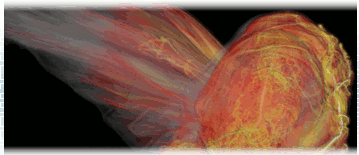
\includegraphics[height=.875cm]{figs/visit-logos/VisIt-03}} \href{https://wci.llnl.gov/simulation/computer-codes/visit/}{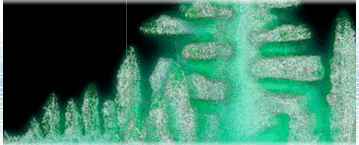
\includegraphics[height=.875cm]{figs/visit-logos/VisIt-04}} \hspace{-8.5cm}{\bf \textcolor{white}{VisIt}}}

\begin{columns}
\begin{column}{5.5cm}
\begin{itemize}
        \item can run: locally, remotelly, client/server mode
        \item interface pretty much looks the same on each platform
        \item can read over a 120 different data formats (\ding{223} \href{http://www.visitusers.org/index.php?title=Detailed_list_of_file_formats_VisIt_supports}{\small detailed list of file formats})
        \item new database plugin readers can be developed
\end{itemize}
\pause
\begin{beamerboxesrounded}[upper=block head,lower=block body,shadow=true]{\ding{232} Supported \textcolor{DarkRed}{Mesh Types} }
        \ding{231}~\textcolor{DarkBlue}{1D Curves}

        \ding{231}~\textcolor{DarkBlue}{2D/3D meshes}: Rectilinear, Curvilinear, Unstructured, Points, AMR, Molecular, CSG
\end{beamerboxesrounded}
\end{column}
\begin{column}{6.25cm}
\pause
\begin{beamerboxesrounded}[upper=block head,lower=block body,shadow=true]{\ding{232} VisIt \textcolor{DarkRed}{Architecture} }
        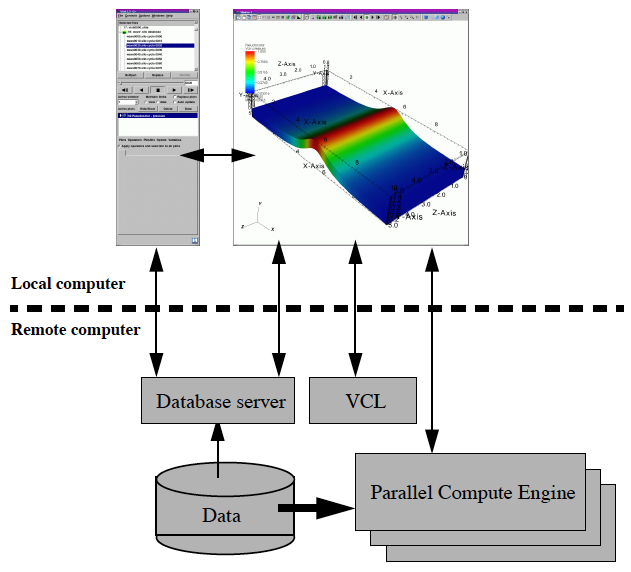
\includegraphics[width=\columnwidth]{figs/visit-guis/VisIt_arch}
\end{beamerboxesrounded}
\end{column}
\end{columns}

\end{frame}



\begin{frame}
\frametitle{\href{https://wci.llnl.gov/simulation/computer-codes/visit/}{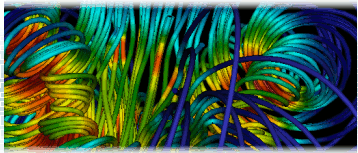
\includegraphics[height=.85cm]{figs/visit-logos/VisIt-01}} \hspace{-.85cm}{\bf \textcolor{white}{VisIt}}: Multiple Interfaces}

\begin{columns}
\begin{column}{4.75cm}
\begin{itemize}
        \item GUI (graphical user interface)
        \item Python programming interface
        \item Java programming interface
        \item C++ programming interface
\end{itemize}
\end{column}
\begin{column}{7.25cm}
\pause
\begin{beamerboxesrounded}[upper=block head,lower=block body,shadow=true]{\ding{231} Use multiple interfaces simultaneously}
        \ding{232}~Use VisIt as an application or a library

        \ding{232}~C++, Python, Java interfaces allow other applications to control VisIt
\end{beamerboxesrounded}
\end{column}
\end{columns}
\end{frame}


\subsection{GUIs}
\begin{frame}
\frametitle{\href{https://wci.llnl.gov/simulation/computer-codes/visit/}{\href{https://wci.llnl.gov/simulation/computer-codes/visit/}{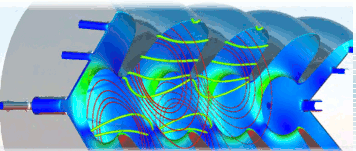
\includegraphics[height=.875cm]{figs/visit-logos/VisIt-02}} {\bf \textcolor{lightgray}{VisIt}}}: GUI}

\begin{columns}
\begin{column}{5.5cm}
\pause
\begin{beamerboxesrounded}[upper=block head,lower=block body,shadow=true]{\ding{232}  \textcolor{DarkRed}{GUI} }
        \textcolor{DarkRed}{\ding{223}} Select files to visualize

        \textcolor{DarkRed}{\ding{223}} Create and manage plots

        \textcolor{DarkRed}{\ding{223}} Set plot attributes

        \textcolor{DarkRed}{\ding{223}} Add operators

        \textcolor{DarkRed}{\ding{223}} Set look and props. for visualization
\end{beamerboxesrounded}
\pause
\begin{beamerboxesrounded}[upper=block head,lower=block body,shadow=true]{\ding{232} \textcolor{DarkBlue}{Viewer} }
        \textcolor{DarkBlue}{\ding{223}} display all of the data being visualized

        \textcolor{DarkBlue}{\ding{223}} Mouse navigation

        \textcolor{DarkBlue}{\ding{223}} up to 16 vis windows

        \textcolor{DarkBlue}{\ding{223}} Popup menu

        \textcolor{DarkBlue}{\ding{223}} Toolbars
\end{beamerboxesrounded}
\end{column}
\begin{column}{6cm}
        \centering
        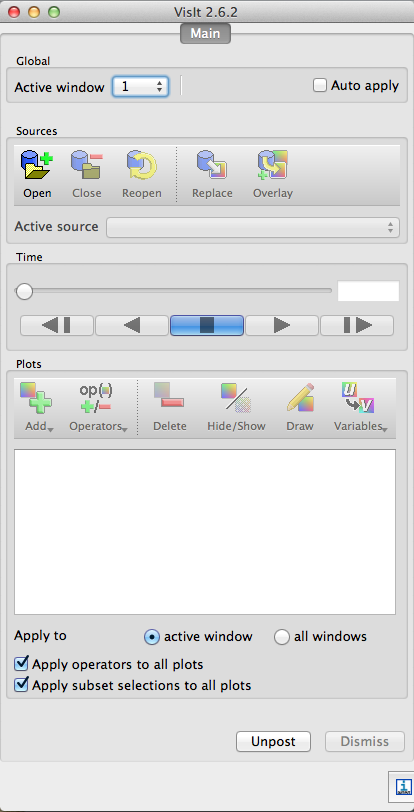
\includegraphics[width=.3\columnwidth]{figs/visit-guis/VisIt_GUI}
        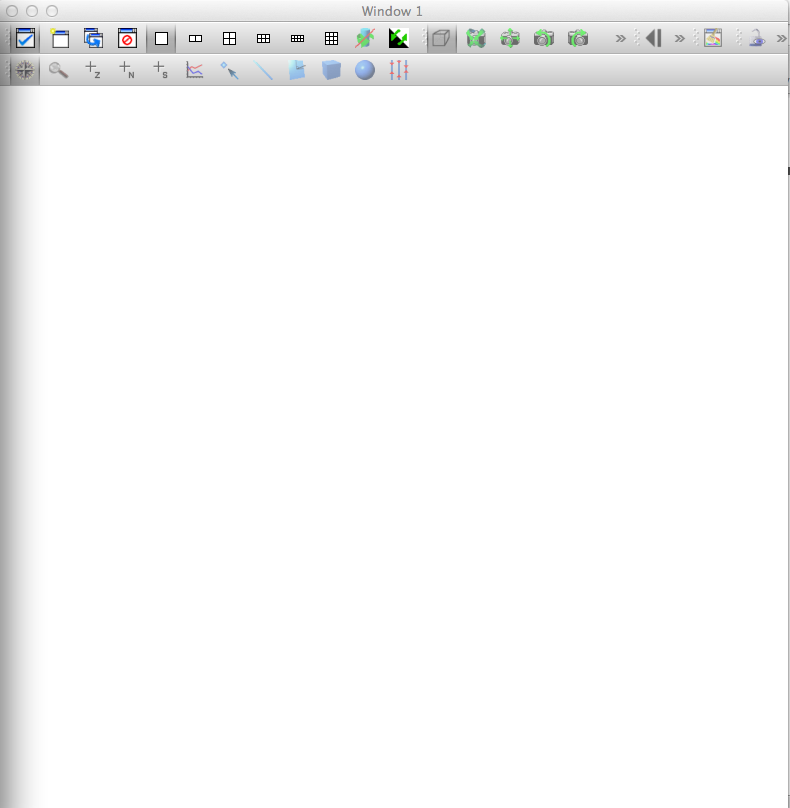
\includegraphics[width=.575\columnwidth]{figs/visit-guis/VisIt_viewer}

        \vspace{2mm}
        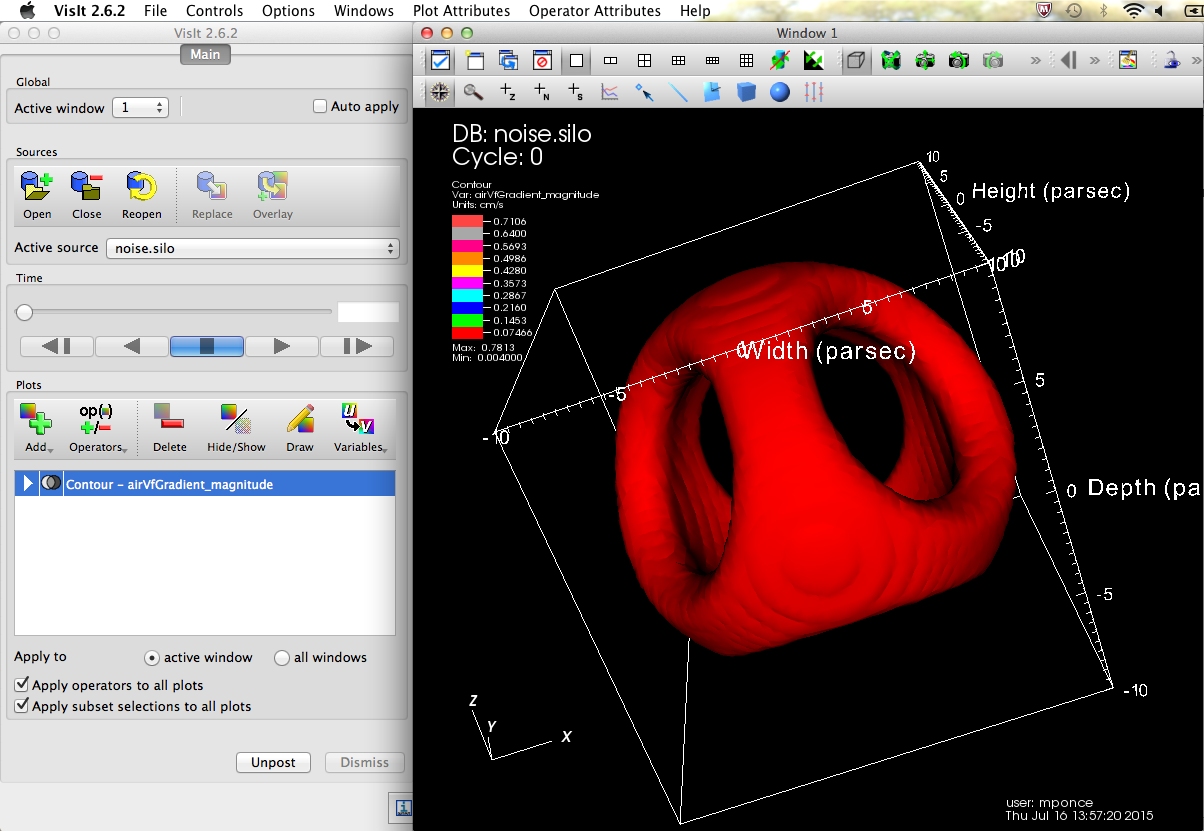
\includegraphics[width=\columnwidth]{figs/visit-guis/VisIt_windows}
\end{column}
\end{columns}
\end{frame}


\begin{frame}
\frametitle{\href{https://wci.llnl.gov/simulation/computer-codes/visit/}{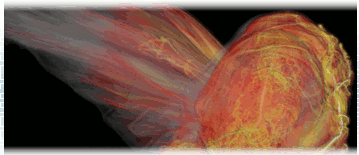
\includegraphics[height=.85cm]{figs/visit-logos/VisIt-03}} \hspace{-.85cm}{\bf \textcolor{lightgray}{VisIt}}: GUIs}

\begin{columns}
\begin{column}{5cm}
\begin{beamerboxesrounded}[upper=block head,lower=block body,shadow=true]{\ding{224}  \textcolor{DarkRed}{Main window in GUI} }

        \textcolor{DarkRed}{\ding{223}} Access other important windows

        \textcolor{DarkRed}{\ding{223}} Open files

        \textcolor{DarkRed}{\ding{223}} Set animation time state

        \textcolor{DarkRed}{\ding{223}} Set active window

        \textcolor{DarkRed}{\ding{223}} Create and manage filters (pipeline)

        \textcolor{DarkRed}{\ding{223}} Displays progress from compute engine
\end{beamerboxesrounded}

\pause
\vspace{1mm}
\begin{beamerboxesrounded}[upper=block head,lower=block body,shadow=true]{\ding{231} Really useful ones}
        \hspace{1.25mm}
        \textcolor{DarkBlue}{\ding{232} Apply to... } check-boxes
\end{beamerboxesrounded}
\end{column}
\begin{column}{6cm}
        \centering
        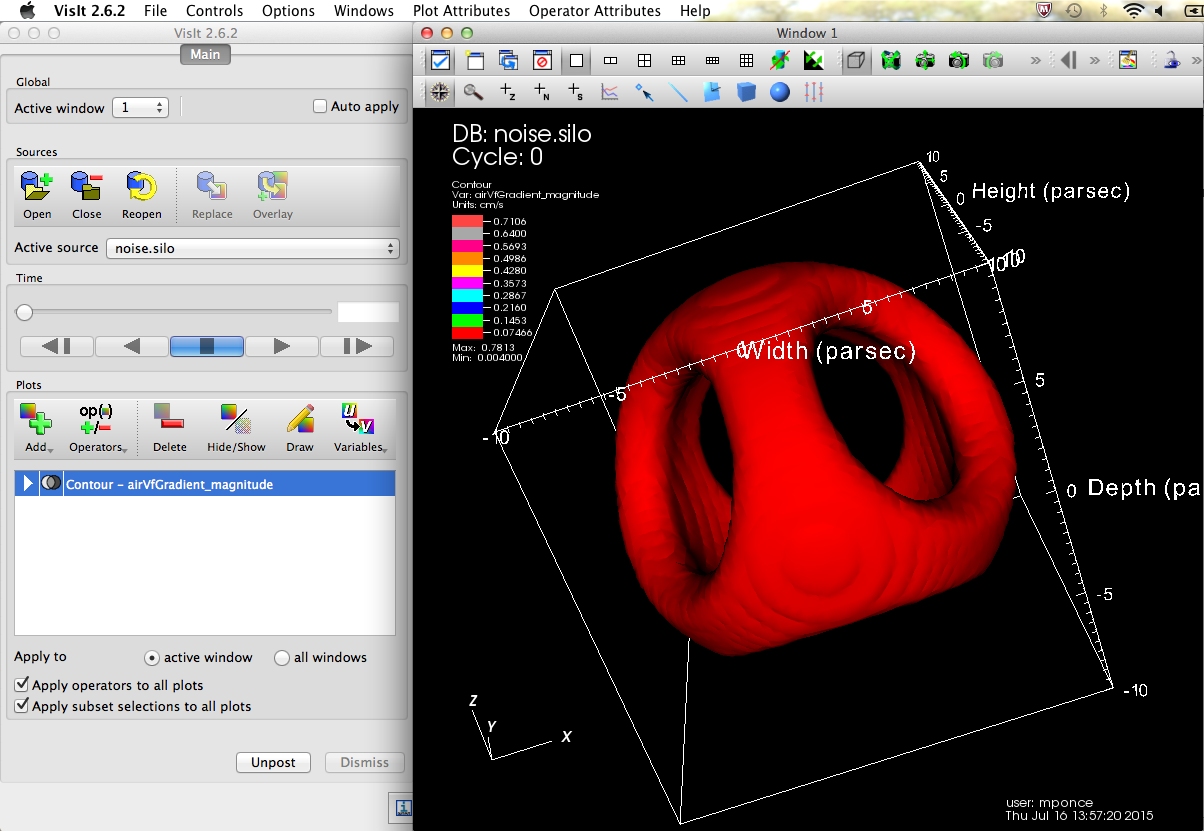
\includegraphics[clip=true,trim=0 0 17cm 0, width=.85\columnwidth]{figs/visit-guis/VisIt_windows}
\end{column}
\end{columns}
\end{frame}


\begin{frame}
\frametitle{\href{https://wci.llnl.gov/simulation/computer-codes/visit/}{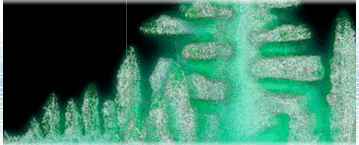
\includegraphics[height=.85cm]{figs/visit-logos/VisIt-04}} \hspace{-.85cm}{\bf \textcolor{white}{VisIt}}: GUIs}

\vspace{-3mm}
\begin{columns}
\begin{column}{5cm}
\begin{beamerboxesrounded}[upper=block head,lower=block body,shadow=true]{\ding{224}  \textcolor{DarkBlue}{Main Menu} }

        \textcolor{DarkBlue}{\ding{223}} \framebox{File}

        \textcolor{DarkBlue}{\ding{223}} \framebox{Controls}

        \textcolor{DarkBlue}{\ding{223}} \framebox{Options}

        \textcolor{DarkBlue}{\ding{223}} \framebox{Windows}

        \textcolor{DarkBlue}{\ding{223}} \framebox{Plot Attributes}

        \textcolor{DarkBlue}{\ding{223}} \framebox{Operator Attributes}

        \textcolor{DarkBlue}{\ding{223}} \framebox{Help}
\end{beamerboxesrounded}
\end{column}
\begin{column}{6cm}
        \centering
        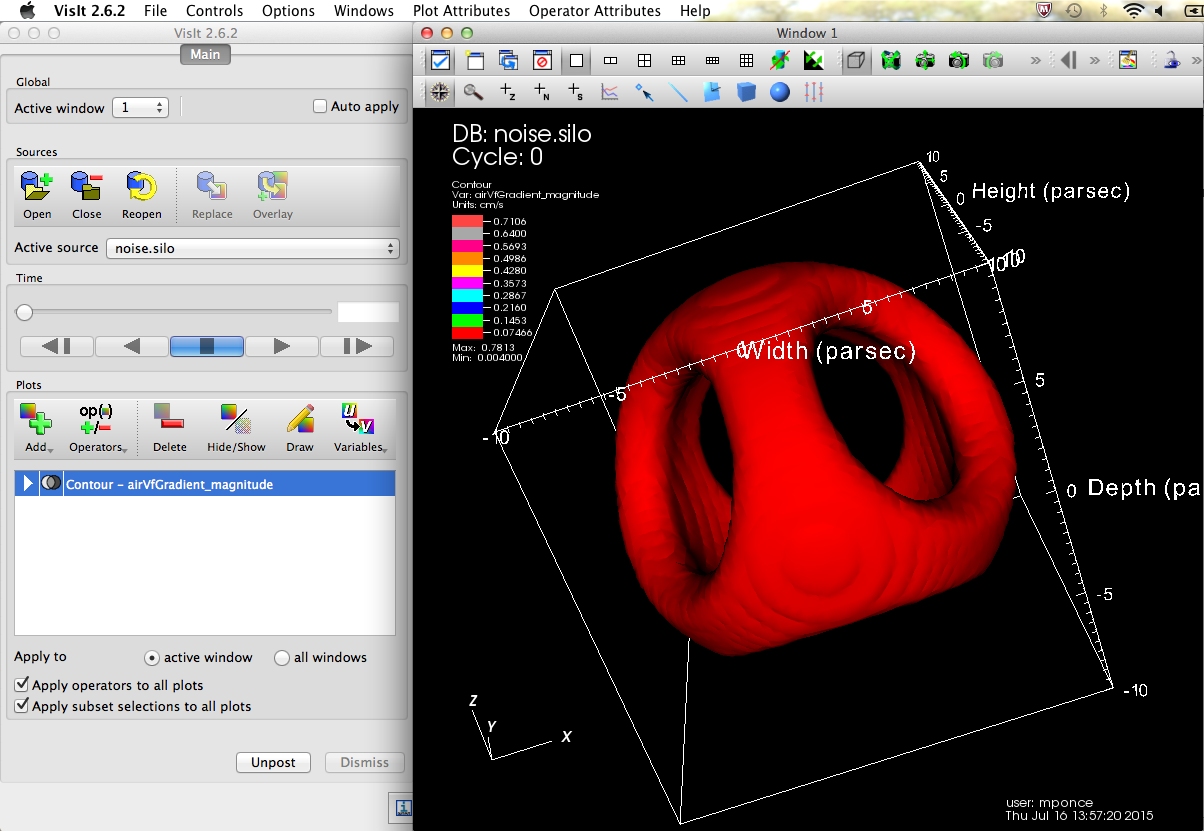
\includegraphics[clip=true,trim=0 0 17cm 0, width=.85\columnwidth]{figs/visit-guis/VisIt_windows}
\end{column}
\end{columns}

\begin{beamerboxesrounded}[upper=block head,lower=block body,shadow=true]{\ding{224}  \textcolor{DarkBlue}{Visualization Toolbar} }
        \centering
        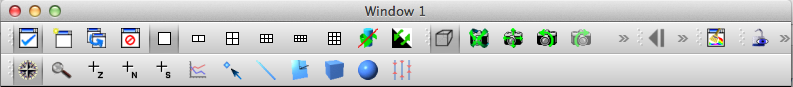
\includegraphics[width=.85\columnwidth]{figs/visit-guis/VisIt_toolbar}
\end{beamerboxesrounded}
\end{frame}


\subsection{Viz Pipeline}
\begin{frame}
\frametitle{\href{https://wci.llnl.gov/simulation/computer-codes/visit/}{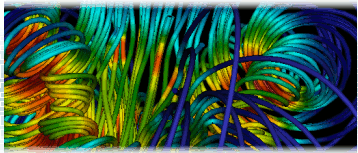
\includegraphics[height=.85cm]{figs/visit-logos/VisIt-01}} \hspace{-.85cm}{\bf \textcolor{lightgray}{VisIt}}: Visualization Pipeline}

\begin{columns}
\begin{column}{5cm}
\begin{beamerboxesrounded}[upper=block head,lower=block body,shadow=true]{}
\begin{enumerate}
        \item Open database (or file)
        \item Create a plot
        \item Set plot attributes
        \item Apply operators to plot to modify data
        \item Set operator attributes
        \item Compute engine generates plot
        \item Plot displayed in vis window
        \item iterate//repeat...
\end{enumerate}
\end{beamerboxesrounded}
\end{column}
\begin{column}{6cm}
        \centering
        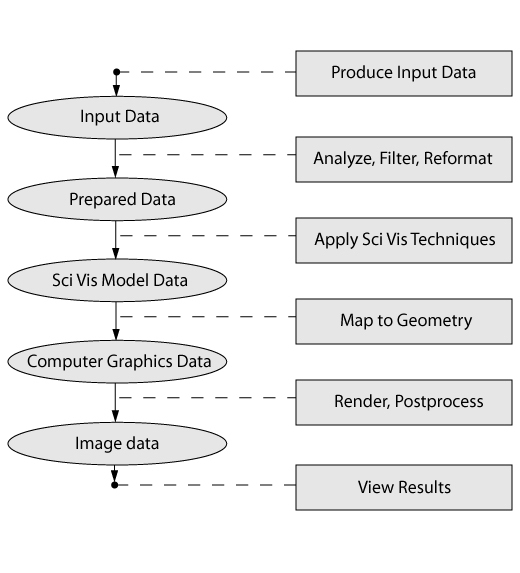
\includegraphics[width=.85\columnwidth]{figs/viz/viz-pipeline4}
\end{column}
\end{columns}

\end{frame}

